\documentclass[12pt,a4paper]{article}
\usepackage[brazilian]{babel}
\usepackage[utf8]{inputenc}
\usepackage[T1]{fontenc}
\usepackage{amsmath,amssymb}
\usepackage{graphicx}
\usepackage{geometry}
\usepackage{hyperref}
\geometry{margin=2.5cm}

\title{Aulas 06 e 06b - Comportamento Exponencial\\Resumo, Exemplo e Exercicios Resolvidos}
\author{Baseado apenas nos arquivos da pasta 5}
\date{14/04/2026}

\begin{document}
\maketitle

\section{Resumo rapido}
Pelo texto legivel em \texttt{pmmat\_aula06.pdf} e \texttt{pmmat\_aula06b.pdf}, os topicos sao:
\begin{itemize}
  \item conceito de funcao exponencial;
  \item crescimento exponencial ($b>1$);
  \item decaimento exponencial ($0<b<1$);
  \item assintota horizontal e comportamento no infinito;
  \item ajuste de dados (mencao a ajuste linear de pontos).
\end{itemize}

\section{Explicacao simples}
Funcao exponencial descreve mudancas que dependem do valor atual.
Se a base e maior que 1, cresce cada vez mais rapido.
Se a base esta entre 0 e 1, decai e se aproxima de zero.
Por isso ela aparece em juros, populacoes, radioatividade e resfriamento.

\section{Exemplo guiado}
Suponha $f(x)=3\cdot 2^x$.
\begin{itemize}
  \item como a base e $2>1$, ha crescimento;
  \item $f(0)=3$, $f(1)=6$, $f(2)=12$;
  \item a funcao aumenta rapidamente quando $x$ cresce.
\end{itemize}

\section{Exercicios dos slides resolvidos passo a passo}
\subsection*{Exercicio 1: classificar crescimento ou decaimento}
Para $f(x)=ab^x$:
\begin{itemize}
  \item se $b>1$, a funcao representa crescimento exponencial;
  \item se $0<b<1$, representa decaimento exponencial.
\end{itemize}

Aplicacao:
\begin{equation}
2\cdot 1.3^x \Rightarrow \text{crescimento},
\qquad
5\cdot 0.7^x \Rightarrow \text{decaimento}.
\end{equation}

\subsection*{Exercicio 2: comportamento assintotico}
Para $f(x)=ab^x$ com $a>0$:
\begin{itemize}
  \item crescimento ($b>1$): $x\to +\infty \Rightarrow f(x)\to +\infty$, e $x\to -\infty \Rightarrow f(x)\to 0$;
  \item decaimento ($0<b<1$): $x\to +\infty \Rightarrow f(x)\to 0$, e $x\to -\infty \Rightarrow f(x)\to +\infty$.
\end{itemize}
A assintota horizontal e $y=0$.

\subsection*{Exercicio 3: montar funcao exponencial por dois pontos}
Suponha $f(0)=3$ e $f(2)=12$ para $f(x)=ab^x$.

De $f(0)=a=3$.

De $f(2)=3b^2=12 \Rightarrow b^2=4 \Rightarrow b=2$ (base positiva).

Logo:
\begin{equation}
f(x)=3\cdot 2^x.
\end{equation}

\subsection*{Exercicio 4: linearizacao para ajuste}
Se $y=ab^x$, tomando logaritmo:
\begin{equation}
\ln y = \ln a + x\ln b.
\end{equation}
Assim, o ajuste exponencial pode ser feito por regressao linear entre $x$ e $\ln y$.

\begin{figure}[htbp]
\centering
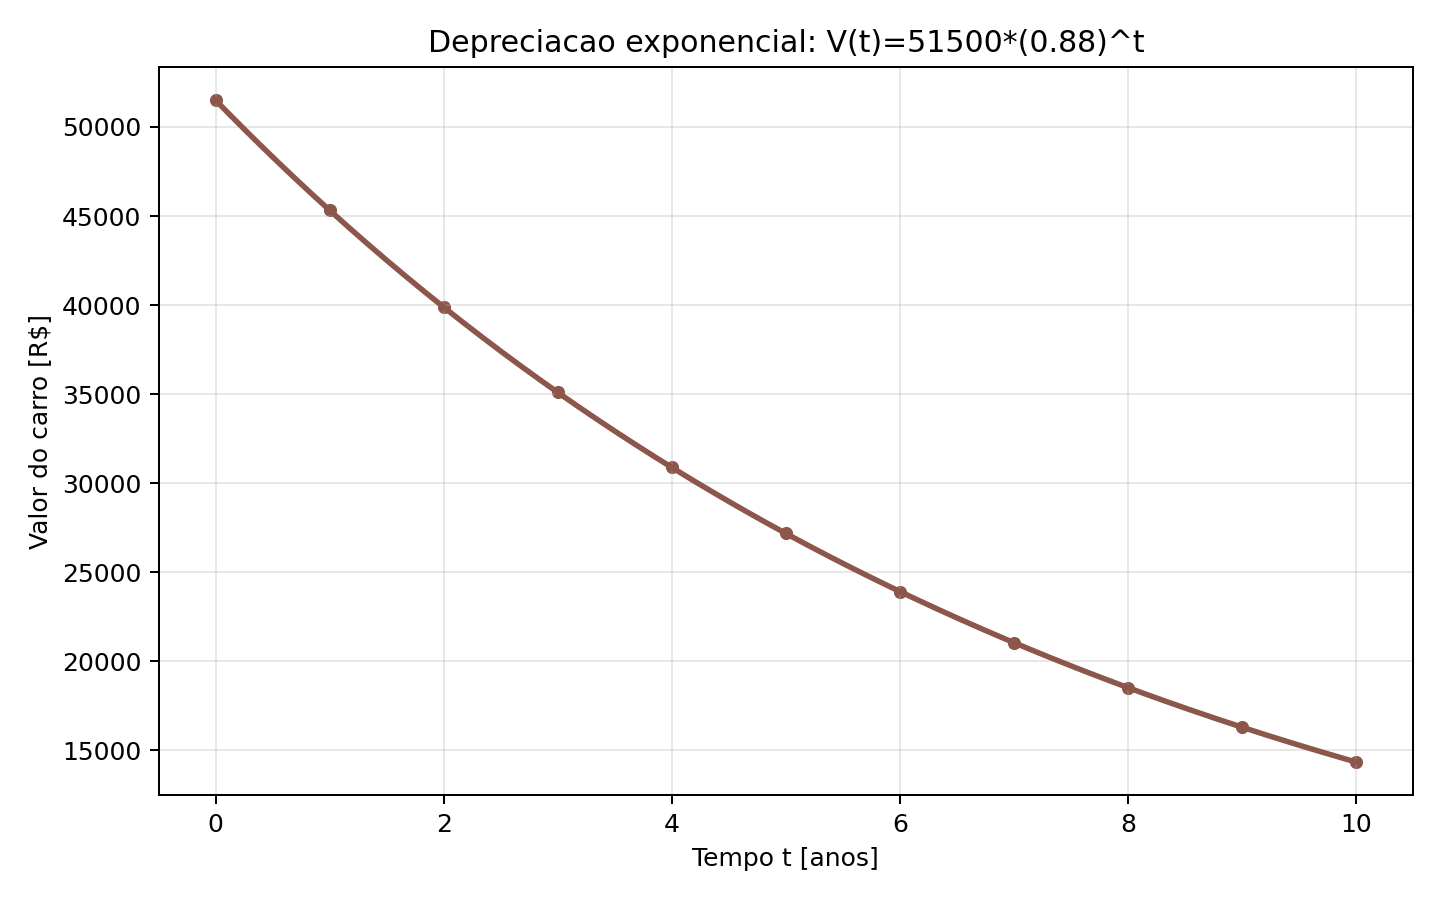
\includegraphics[width=0.8\textwidth]{figuras/depreciacao_exponencial.png}
\caption{Grafico da depreciação exponencial usado nos exercicios.}
\end{figure}

\section{Fontes web para revisar}
\begin{itemize}
  \item Funcao exponencial (conceitos e propriedades): \url{https://pt.wikipedia.org/wiki/Fun%C3%A7%C3%A3o_exponencial}
\end{itemize}

\end{document}
